\documentclass[english,12pt,a4paper,final]{article}
\usepackage[T1]{fontenc}
\usepackage{babel}
\usepackage{graphicx}
\usepackage{amsmath}
\usepackage{amssymb}
\usepackage{relsize}
\usepackage[normalem]{ulem}
\usepackage{xcolor}
\usepackage{parskip}
\usepackage{hyperref}
\usepackage{float}
\usepackage{tikz}
\usetikzlibrary{3d, arrows.meta}
\usepackage[a4paper, total={6.27in, 9.69in}]{geometry}

\definecolor{OliveGreen}{rgb}{0,0.6,0}
\definecolor{firebrick}{rgb}{0.7, 0.13, 0.13}
\definecolor{DarkBlue}{rgb}{0.1, 0.3, 0.5}

\usepackage[backend=biber, style=authoryear]{biblatex}
\addbibresource{bibliography.bib}
\DeclareDelimFormat{nameyeardelim}{\addcomma\space}

\hypersetup{
	colorlinks=true,
	linkcolor=black,
	urlcolor=blue,
	citecolor=firebrick,
	pdftitle={Exploring Variations of Penney's Game},
	pdfauthor={William Dracopoulos}
}

\title{Exploring Variations of Penney's Game}
\author{
William Dracopoulos
\\
John Abbott College
}

\begin{document}

\maketitle
	
\begin{center}

\Large

\includegraphics[width=0.7\linewidth]{"s3k4 3p"}

Independent Research Project in Science

360-RES-AB (Winter 2025)

Research Supervisor: Derrick Chung - John Abbott College

Course Coordinator: Ferenc Balogh

\begin{center}
	
\includegraphics[width=0.27\linewidth]{John-Abbott}
\end{center}

\end{center}

\newpage

\tableofcontents
\newpage

\part{Abstract}

Penney’s Game is an example of where our intuitive understanding of probability completely fails; it’s a seemingly fair game with a surprisingly complicated strategy. The goal of this research is to explore Penney’s Game using new methods and in areas that it has not been explored before. By studying a similar game which is fair, we create a formula for the probability of each player winning Penney’s Game depending on the number of players, the sequences chosen by each player, the length of each sequence, the number of possible outcomes of the “flip” (coin flip or dice roll or random outcome generation), and the probability distribution of the outcomes of this flip. The formula was verified by computer simulations and then packaged into an online probability calculator. This research tool was then used to attract our attention toward patterns within Penney's Game, leading to a few new proofs. Among these, it was proven that games tend towards being fair with an infinite number of possible outcomes from the “flip” but not infinite sequence length, and that the shorter sequence always has an advantage, except in some specific and known cases. The work done in this paper is not exhaustive. There is still plenty to explore and discover, and we leave behind tools to help future researchers to do this.

\part{Introduction}

In its basic variation, Penney's Game is simple game invented by Walter Penney involving two players and one coin. Each player predicts which sequence of flips will appear first as the coin is being flipped. For example, Alice predicts that HHT (heads, then heads, then tails) will appear first, while Bob predicts that THT (tails, then heads, then tails) will appear first. The players flip the coin until the last three coin flips match with the sequence predicted by one of the players. That player wins. Note that this does not mean the coin is flipped three times, a match is checked for, and then it's flipped three times again. Instead, after every coin flip, the last three flips are checked to see if they match with a player's prediction.

The game might seem fair, but it is not. In that example, Alice actually has a 62.5\% chance of beating Bob. In fact, for any sequence that one player predicts, there is another that will beat it on average \parencite{penney}. A formula for finding the exact win probabilities for any sequence in this basic variation of the game (the variation being described) was first discovered by the mathematician John Conway, but he never supplied a proof of his "leading number algorithm".

Since Conway, many other researchers have developed different algorithms and ways of thinking about the problem. One way is using Markov chains and martingale arguments, such as the paper by \textcite{markov}. However, we use a much simpler way of understanding the game and deriving a formula for win probabilities. The general idea, which will be explained in depth during Part \ref{derivingFormula2P}, is to think about another game instead, which this time is always fair. This new game, which we will call the betting game, contains the same probabilities as Penney's Game but has a clear and powerful starting point for analysis due to its fairness. The idea of the betting game comes simultaneously from two places: a research paper which tackles Penney's game from the perspective of no-arbitrage \parencite{miller}, and \textcite{chung}'s talk which describes it in the context of the Optional Stopping Theorem. The latter will be the same approach used in this paper.

Our goal is to extend the betting game analogy further than ever before to allow us to determine probabilities in many variations of Penney's Game. A formula, \eqref{generalFormula}, will be derived which can calculate the win probabilities in games with:

\begin{enumerate}
	\item Any number of players
	\item Players predicting any number of flips in the future, even if this number is different for each player
	\item Any kind of coin, die, or random outcome generator being "flipped"
	\item Unfair coins, loaded dice, and random outcome generators with any probability distribution
\end{enumerate}

We also verify our formula with simulations, and then analyze it to discover new things about Penney's Game in some of the variations covered by the formula.

\part{Showing that Penney's Game is unintuitive, and providing some hints for understanding it}

Penney's game was introduced as seeming fair but actually being biased. However, in some cases it seems like one player should be advantaged, while in reality the game is completely fair.

Imagine someone sitting at a table and flipping a coin until there are three consecutive heads. They will find that, on average, HHH appears after the 14th coin flip. Now they do the same and count how many flips it takes to get HHT. This time, they count that HHT appears after only the 8th coin flip on average. We went through this process and collected data for each sequence in the basic variation, which is shown in Figure \ref{fig:probGraph}.

\newpage

\begin{figure}
	\centering
	\includegraphics[width=0.7\linewidth]{"./prob graph"}
	\caption{Probability of a sequence appearing for the first time as a function of the number of coin flips passed. The data was obtained from a simulation of 1 000 000 repetitions. The expected wait time (number of flips until the sequence appears) for the purple, black, and green lines are calculated to be approximately 8 flips, 10 flips, and 14 flips respectively.}
	\label{fig:probGraph}
\end{figure}

An exact function for the green line was found by my friend Fenghua Li to be 
\begin{equation*}
	\mathbb{P}_n=\frac{1}{16} A
\end{equation*}
\begin{equation*}
	A = \frac{1}{2^m}\sum_{s=0}^{m- \lfloor \frac{m}{3} \rfloor}\sum_{L=\lceil \frac{s}{2} \rceil}^{s} {m+1-s \choose L} {L \choose s-L} \text{ with } m=n-4
\end{equation*}
This gives the probability of the sequence appearing ($\mathbb{P}$) for any number of previous coin flips ($n$) in the cases of HHH and TTT.

This might lead one to believe that HHT would beat HHH in Penney's Game, since it would appear earlier, but in fact HHT vs. HHH would be a fair game. Figure \ref{fig:probGraph} does not provide enough information to make conclusions about Penney's Game. It does not take into account how the sequences interact with each other. The difference is that the expected wait time as shown in Figure \ref{fig:probGraph} comes from one player flipping one coin, but in Penney's Game, it's two players checking for their sequence on the same coin. Imagine the last two coin flips were heads. There is now a 50:50 chance that the third flip will land on heads and tails. Therefore it is equally likely that HHT and HHH appears, so the game is fair.

The situation is very different if you switch it around to be THH vs. HHH. This will actually give the greatest probability difference in the basic variation of the game: the player predicting HHH will only have a 12.5\% (or $\frac{1}{8}$) chance of winning. This is because as soon as a single coin flip lands on tails, HHH has no chance of appearing before THH; THH will always get to two heads in a row before HHH gets to three in a row. This leaves only one way for HHH to win: if the first three coin flips land on heads, which is a $\frac{1}{2^3} = \frac{1}{8}$ chance.

We have shown that Penney's Game is unintuitive but not impossible to understand. Now we can move on to analyzing it through the betting game to develop a general formula for win probabilities.

\part{Deriving a formula for win probabilities with two players}\label{derivingFormula2P}

\section{The basic variation of Penney's Game}

Imagine two players sitting at a table with one coin between them. Each player picks a sequence and they begin to flip the coin until the last flips match with one of the player's sequences. Up until now, the game has been identical to Penney's Game, and that is by design. Now it begins to differ. This is how the betting game works:

Right before each coin flip, both players bet on their chosen sequence appearing in the next flips. This means each player will likely have multiple bets going on at the same time, since a new sequence of bets starts for each flip, and each sequence might last for multiple flips (if it doesn't get interrupted, it will last for three). They are also always betting on the same chosen sequence throughout the game. The bets are against each other; there is no third party that gives or takes money, so if one wins \$2, it's the other player that gives it to them. Although the game ends when one player's sequence appears in the flips, there is no winner nor loser, just an exchange of money.
\\\\
We will explain using an example: Let's say Alice chooses HHT and Bob chooses THT. We'll start by following only the sequence of bets that starts from the first flip. 

Before the coin is flipped for the first time, Alice bets that the flips will follow her sequence, so she bets that the first will be H, the second H, and the third T. Bob simultaneously bets that the first flip will be T, the second H, and the third T. 

Both players start each sequence of bets by betting \$1 on the first flip of the sequence. If they win, they will have \$2 which they will use to bet on the second flip, and so on, doubling each time. If they lose any bet, all the money they wagered will be gone and this sequence of bets will end. 

By random chance, the first coin lands on heads. Alice now has \$2 and Bob has lost the bet: his prediction has failed and he lost the \$1 to Alice. He also has to pay \$1 to Alice for her win. So she actually has \$3 and he has -\$1. 

Bob's sequence of bets is finished, but Alice continues. She bets the \$2 from her win on the next flip being heads. They flip the coin again and it lands on heads. Alice  now has \$5 after winning another \$2 from Bob, who went to -\$3. 

Alice bets the \$4 from her correct bets so far on tails to finish her sequence of HHT. The third flip lands on heads instead, so Alice loses that \$4 to Bob, and they start back where they began: each has \$1.

There can be any number of ineffective sequences of bets like this until the game ends. But remember that each time a coin was flipped, each player starts new bets on their chosen sequence of flips. There were bets that we haven't looked at yet.

This hypothetical game ends one flip later, with Alice's sequence appearing in the coin flips. We will illustrate this game in a table. The top row represents the coin flips that actually occur. All other rows represent a new sequence of bets that the player makes. The columns show all bets made simultaneously before each flip, although all bets will be for different amounts of money. Notice that the row labelled 1 shows the sequence of bets that we described previously: the sequence that starts at the first coin flip. But there were three more sequences of bets until the game ended.

To simplify, we can think of the bets slightly differently. We can ignore the constant exchange of money between players, and have them keep track of their profit so that they exchange money only at the end of the game.
\\\\\\
Alice:
\begin{tabular}{|c|c|c|c|c|}
	\hline
	& H & H & H & T \\
	\hline
	1 & \textcolor{OliveGreen}{H} & \textcolor{OliveGreen}{H} & \textcolor{red}{\sout{T}} &  \\
	\hline
	2 &  & \textcolor{OliveGreen}{H} & \textcolor{OliveGreen}{H} & \textcolor{OliveGreen}{T} \\
	\hline
	3 &  &  & \textcolor{OliveGreen}{H} & \textcolor{red}{\sout{H}} \\
	\hline
	4 &  &  &  & \textcolor{red}{\sout{H}} \\
	\hline
\end{tabular}
\\\\\\
We colour the successful bets in green and the unsuccessful ones in red. Alice has a single sequence of bets that was successful: row 2. From it, she is at \$8 because her three bets in a row were successful, also meaning that Alice made the game end. From the other sequences, she has nothing. So we can say that Alice has \$8 and therefore Bob owes her \$8. But during this time, what was Bob doing?
\\\\\\
Bob:
\begin{tabular}{|c|c|c|c|c|}
	\hline
	& H & H & H & T \\
	\hline
	1 & \textcolor{red}{\sout{T}} & H & T &  \\
	\hline
	2 &  & \textcolor{red}{\sout{T}} & H & T \\
	\hline
	3 &  &  & \textcolor{red}{\sout{T}} & H \\
	\hline
	4 &  &  &  & \textcolor{OliveGreen}{T} \\
	\hline
\end{tabular}
\\\\\\
In all rows except 4, Bob loses the sequence of bets immediately. So all others after it are not coloured, indicating that they don't have an opportunity to happen at all. He won the first bet in row 4, but this sequence of bets was cut off by Alice winning her three bets in a row and ending the game, meaning that Bob got to keep the \$2 he won from row 4.

In total, Bob owes Alice \$8, but Alice owes Bob \$2. After the exchange, Alice has profited \$6 and Bob has lost \$6.

If, in another game, either player had received money from a sequence of bets which started at another flip, the money would get added to the total before the exchange.

It is very important to notice that the final share of money is not unique to this game in particular. In any game where Alice's sequence of HHT appears before Bob's sequence of THT, Alice will end up getting \$6 from Bob. This is because all of the flips before the last three do not matter: the prior bets of both Alice and Bob will fail eventually. The only two ways for a player to make money from a sequence of bets are:

\begin{enumerate}
	\item If the bets go to completion. In other words, if the three bets in a row succeed. This will end the game.
	\item If a sequence of bets gets cut off by the game ending.
\end{enumerate}

We can ignore all sequences of bets before the last three because we know they won't give anyone any money. They can't return money in the first way because if they did, the game would be over already. And we cover all bets that might return money in the second way by including the two sequences of bets that get cut off (the last two).

We can now introduce a better version of the table, which we will use throughout the paper.
\\\\\\
$R_A(A)$:
\begin{tabular}{|ccc|c|}
	\hline
	H & H & T & Gain \\
	\hline
	
	\textcolor{OliveGreen}{H} & \textcolor{OliveGreen}{H} & \textcolor{OliveGreen}{T} & $2^3=8$ \\
	
	& \textcolor{OliveGreen}{H} & \textcolor{red}{\sout{H}} & $0$ \\
	
	&  & \textcolor{red}{\sout{H}} & $0$ \\
	\hline
\end{tabular}
$=8$
\\\\\\
It now only features the important rows: the last 3. And it shows that Alice's (denoted by the $A$ within the parentheses) "return" ($R$) when her own sequence appears (denoted by the $A$ in the subscript) will be \$8.

The same table can be made for Bob's return when Alice's sequence appears:
\\\\\\
$R_A(B)$:
\begin{tabular}{|ccc|c|}
	\hline
	H & H & T & Gain \\
	\hline
	
	\textcolor{red}{\sout{T}} & H & T & $0$ \\
	
	& \textcolor{red}{\sout{T}} & H & $0$ \\
	
	&  & \textcolor{OliveGreen}{T} & $2$ \\
	\hline
\end{tabular}
$=2$
\\\\\\\\\\
We have found all we need to know about what happens when Alice's sequence appears. Now let's focus on when Bob's sequence appears, by making the tables:
\\\\\\
$R_B(A)$:
\begin{tabular}{|ccc|c|}
	\hline
	T & H & T & Gain \\
	\hline
	
	\textcolor{red}{\sout{H}} & H & T & $0$ \\
	
	& \textcolor{OliveGreen}{H} & \textcolor{red}{\sout{H}} & $0$ \\
	
	&  & \textcolor{red}{\sout{H}} & $0$ \\
	\hline
\end{tabular}
$=0$
\\\\\\
So Alice makes \$0 from Bob when his sequence appears in the coin flips.
\\\\\\\\

$R_B(B)$:
\begin{tabular}{|ccc|c|}
	\hline
	T & H & T & Gain \\
	\hline
	
	\textcolor{OliveGreen}{T} & \textcolor{OliveGreen}{H} & \textcolor{OliveGreen}{T} & $8$ \\
	
	& \textcolor{red}{\sout{T}} & H & $0$ \\
	
	&  & \textcolor{OliveGreen}{T} & $2$ \\
	\hline
\end{tabular}
$=10$
\\\\\\
And Bob makes \$10 from Alice when his sequence appears in the coin flips.
\\\\
In total, when Bob's sequence appears, Alice gives him \$10.

Note that something interesting is happening here. When Alice's sequence appears, Alice makes \$6 from Bob, but when Bob's sequence appears, he makes \$10 from Alice. This might make it seem like Bob has an advantage in this game, but there's a problem with that.
\\\\
\textbf{Here is the point of all this:} All Alice and Bob are doing is betting on a fair coin, and either doubling or losing the money they put into the bet. Each individual bet is \underline{fair}. But because of the linearity of expectation, it doesn't matter if you make a fair bet once or 100 times, on average, you should expect to neither lose nor gain money. Your expected profit should be 0.

But it seems like Bob is doing better than Alice, and that doesn't make sense \textit{assuming} that Bob's sequence and Alice's sequence have an equal chance of appearing. So let's simply assume that they don't. We'll take $\mathbb{P}(A)$ to mean the probability that Alice's sequence appears and ends the game, and $\mathbb{P}(B)$ to mean the probability that Bob's sequence appears and ends the game.

Let's look at it from Alice's perspective:

\begin{equation*}
	(\$6) \cdot \mathbb{P}(A)  + (-\$10) \cdot \mathbb{P}(B) = \$0
\end{equation*}

In words, Alice's net profit when her sequence appears (\$6) weighed by the chance that her sequence appears ($\mathbb{P}(A)$), added to Alice's net profit when Bob's sequence appears (-\$10) weighed by the chance that his sequence appears ($\mathbb{P}(B)$) is her expected profit, which for the reason explained above must be exactly \$0.

Now, of course, either Alice's or Bob's sequence must appear, so

\begin{equation}\label{PA+PB=1}
	\mathbb{P}(A) + \mathbb{P}(B) = 1
\end{equation}

We now have two equations and two unknowns, so $\mathbb{P}(A)$ and $\mathbb{P}(B)$ can be found. After some algebra, $\mathbb{P}(A) = 62.5\%$ and $\mathbb{P}(B) = 37.5\%$.

Importantly, this means that if Alice and Bob were playing Penney's Game with the sequences HHT and THT, Alice would have a 62.5\% chance of winning and Bob would have a 37.5\% chance of winning. This is because Penney's Game and the betting game end in exactly the same way, \textbf{so $\mathbb{P}(A)$ and $\mathbb{P}(B)$ apply to Penney's Game too}.

Generalizing beyond this example, we can define the net profit of Player X against Player Y when sequence Z appears (Z being either Player X or Player Y's sequence) as:

\begin{equation}\label{NtwoPlayers}
	N_Z(X) = R_Z(X) - R_Z(Y)
\end{equation}

Next, we can solve for $\mathbb{P}(A)$ and $\mathbb{P}(B)$ generally. From the perspective of Player A:

\begin{equation}\label{profitEquation2P}
	N_A(A)\cdot\mathbb{P}(A) + N_B(A)\cdot\mathbb{P}(B) = 0
\end{equation}

Solving this with the help of \eqref{PA+PB=1}, we get

\begin{equation}\label{PtwoPlayersFirst}
	\mathbb{P}(A) = \frac{-N_B(A)}{N_A(A)-N_B(A)} = \frac{R_B(B)-R_B(A)}{R_A(A)-R_A(B)+R_B(B)-R_B(A)}
\end{equation}

And the formula for $\mathbb{P}(B)$ is exactly the same but with all A and B's swapped. This is exactly the same result as found by Miller and it is equivalent to Conway's leading number algorithm \parencite{miller}.

The last and most complicated thing to do is express the return values $R$ mathematically. The return in \$ for sequence $Y$ if the game ends by sequence $X$ appearing can be given by this equation, which simply describes the process done in the tables above:

\begin{equation}\label{Rbasic}
	R_X(Y) = \sum_{i=1}^{3} \prod_{j=1}^{i} 2_{[Y_j = X_{3-i+j}]}
\end{equation}

Where $2_{[Y_j = X_{3-i+j}]}$ is defined as:
\begin{equation*}
	2_{[Y_j = X_{3-i+j}]} = \begin{cases}
		2 & \text{if } Y_j = X_{3-i+j} \\
		0 & \text{if } Y_j \neq X_{3-i+j} \\
	\end{cases}
\end{equation*}

And the subscript of a sequence indexes its elements. For example, in $X$: HTT, $X_1$ = H; $X_2$ = T; $X_3$ = T.

\eqref{Rbasic} is a specific case of Miller's formula for $R$.

\section{Allowing for any random outcome generator with any known probability distribution}

We have described Penney's Game as being played with a fair coin, but this is not necessary. We can extend the formula to account for any random outcome generator with any known probability distribution. For example, a random outcome generator can be a loaded 20-sided die or a coin flipped in a certain way so that it's more likely to land on heads\footnote{We provide a way to physically model loaded die and unfair coins in Part \ref{physicalModelling}.}. We will generalize all of these random outcome generators by imagining them as a random number generator that outputs integers $[0, 1, ..., n-1]$ for $n$ possible outcomes of the "flip". For example, instead of writing "heads" / "H" and "tails" / T" for a coin, we will write "0" and "1" because a coin has $n=2$. HHT will be written 001. A 6-sided die will be thought of as a generator outputting numbers $0, 1, 2, 3, 4, 5$.

To keep the betting game a valid analogy to Penney's Game, we need to keep the condition that the game must be fair, no matter which outcome generator is being used. This has a simple fix.

The expected profit of a bet must be \$0 for the game to be fair, so

\begin{equation*}
	W \cdot \mathbb{P}(W) + L \cdot \mathbb{P}(L)=0
\end{equation*}

Meaning that the net profit from winning ($W$) weighted by the probability of winning ($\mathbb{P}(W)$), added to the net profit from losing ($L$) weighted by the probability of losing ($\mathbb{P}(L)$) should be zero. Since this bet must either be won or lost, $\mathbb{P}(W) + \mathbb{P}(L) = 1$, so $\mathbb{P}(L) = 1-\mathbb{P}(W)$.

With a fair two-sided coin. We said that each bet is a double-or-nothing. This is because for a bet in which you put $\$X$, there is a 50\% chance of winning $\$X$ and a 50\% chance of losing $\$X$. Therefore $W=X$, $\mathbb{P}(W)=\mathbb{P}(L)=\frac{1}{2}$, and $L=-X$.

\begin{equation*}
	X \cdot \frac{1}{2} + (-X) \cdot \frac{1}{2}=0
\end{equation*}

Now we can generalize for any $\mathbb{P}(W)$. We will say that the outcome of any bet will either be losing what you put into it, $L=-X$, or winning some multiple of what you put into it, $W=\lambda X$. We want to see which multiple $\lambda$ must be used to keep the game fair.

\begin{equation*}
	(\lambda X) \cdot \mathbb{P}(W) + (-X) \cdot (1-\mathbb{P}(W)) = 0
\end{equation*}

\begin{equation*}
	\lambda = \frac{1}{\mathbb{P}(W)} - 1
\end{equation*}

In our table and our formula for $R$, we don't care about how much gets added to the profit, but instead how much profit a player has made after a win. So after winning a bet of $X$, we will be left with a sum of $X'$ such that

\begin{equation*}
	\mathbf{X'} = X + \lambda X = X + \frac{X}{\mathbb{P}(W)} - X = \mathbf{X\frac{1}{\mathbb{P}(W)}}
\end{equation*}

So instead of a double or nothing, it must be a \textit{multiply your bet by $\frac{1}{\mathbb{P}(W)}$} or nothing. We can now include this new rule in our formula for $R$. Replacing the 2 in \eqref{Rbasic} by $\frac{1}{\mathbb{P}(W)}$, we get:

\begin{equation}\label{RanyRandom}
	R_X(Y) = \sum_{i=1}^{3} \prod_{j=1}^{i} \frac{1_{[Y_j = X_{3-i+j}]}}{\mathbb{P}(Y_j)}
\end{equation}

$\mathbb{P}(Y_j)$ is written instead of $\mathbb{P}(W)$ because, in this formula, the bet is always being placed on the $j^{\text{th}}$ element of sequence $Y$ appearing, which we define to be $\mathbb{P}(Y_j)$. \textbf{So $\mathbb{P}(Y_j)$ represents the probability of winning for any bet.} For example, with a fair coin, if sequence Y is HHT and this bet has the index $j=2$, then $\mathbb{P}(Y_j) = \mathbb{P}(H) = \frac{1}{2} = \mathbb{P}(W)$ and we return to what we had in \eqref{Rbasic} because $\frac{1}{(\frac{1}{2})} = 2$.

\section{Extending to games with sequences of different lengths}

As it was previously discussed, a sequence of bets can only return money (and therefore only matter) if either of these things happen:
\begin{enumerate}
	\item The bets go to completion. In other words, if all bets in the sequence succeed. This will end the game.
	\item A sequence of bets gets cut off by the game ending.
\end{enumerate}

This allowed us to only look at the last 3 sequences of bets in the basic variation, because there will be 3 bets going on when the game ends, because the sequences predict the next 3 flips. For a game involving sequences of length $k$, all we have to change is that we should now look at the last $k$ sequences of bets before a player ends the betting. This is again a simple fix in the formula for $R$, introducing a $k$ in the place of the 3:

\begin{equation}\label{RanyLength}
	R_X(Y) = \sum_{i=1}^{k} \prod_{j=1}^{i} \frac{1_{[Y_j = X_{k-i+j}]}}{\mathbb{P}(Y_j)}
\end{equation}

At this point, our formula for $R$ is identical to the one derived by \textcite{miller}, despite some notation changes.

However, we can make one more small change to allow for games in which the players are predicting a different number of coin flips into the future compared to each other. For a sequence $S$, we will define its length (the number of flips predicted in the future) to be $L_S$.

Using the same logic as before, we find that the number of sequences of bets that must be checked when calculating $R_X(Y)$ must be $k = \text{min}\{L_X, L_Y\}$. Additionally, the subscript of X in $1_{[Y_j = X_{k-i+j}]}$ must continue to involve the length of X, which has been changed from $k$ to $L_X$. This completes our work on $R$:

\begin{equation}\label{Rdef}
	R_{X}(Y) = \sum_{i=1}^{\text{min}\{L_{X}, L_{Y}\}} \prod_{j=1}^{i} \frac{1_{[Y_{j} = X_{L_{X} - i + j}]}}{\mathbb{P}(Y_{j})}
\end{equation}

It is important to note that having two or more sequences of different lengths leaves a lot of room for games which break the formula in some way. For example, 1100 vs. 100 would sometimes be a tie in Penney's Game, since when 1\underline{100} appears, 100 must appear simultaneously. Additionally, 1100 vs. 110 would result in 110 always winning Penney's Game, since 110 will always be completed before \underline{110}0. \eqref{Rdef} does not take these intricacies into account, so the results may be wrong.

Games like this can be dealt with using a rule for picking sequences such as "one sequence must not be contained within another or else the game will be considered invalid."

As an interesting byproduct of the function $R$, calculating $R_X(X)$ will return the expected wait time for sequence $X$.

\part{Deriving a formula for win probabilities in games with any number of players}

The last way that we will generalize our formula is to make it work with any number of players. We will define $n$ to represent the number of players, and we will store the predicted sequences of all players in a list: $\{S_1, S_2, ..., S_n\}$.

The first thing we can do is edit \eqref{NtwoPlayers}. This equation says that in the betting game with two players, money won by one player is paid by the other. We can make this work with more than two players. A way to do this which keeps the game fair for everyone (this is always necessary) is to say that at the end of the game, each player's winnings are paid by all other players equally. For example, in a game with 5 players, if one player wins \$1, all the others will give that player \$0.25 when the game ends. Mathematically, that rule can be expressed like this:

\begin{equation}\label{Ndef}
	N_{X}(Y) = \frac{1}{n-1} \mathlarger{[}nR_{X}(Y) - \sum_{i=1}^{n}R_{X}(S_i)\mathlarger{]}
\end{equation}

The problem that is now left is that there are $n$ players, so there are not just two win probabilities (previously simply $\mathbb{P}(A)$ and $\mathbb{P}(B) = 1-\mathbb{P}(A)$), but $n$ unknown win probabilities.

However, we can generate enough equations to solve for all of them. For each player, the betting game must still be fair. Therefore we can extend the logic used in \eqref{profitEquation2P} to get the equations:

\begin{equation*}
	N_{S_1}(S_\textbf{1}) \cdot \mathbb{P}(S_1) + N_{S_2}(S_\textbf{1}) \cdot \mathbb{P}(S_2) + ... + N_{S_n}(S_\textbf{1}) \cdot \mathbb{P}(S_n) = 0
\end{equation*}

\begin{equation*}
	N_{S_1}(S_\textbf{2}) \cdot \mathbb{P}(S_1) + N_{S_2}(S_\textbf{2}) \cdot \mathbb{P}(S_2) + ... + N_{S_n}(S_\textbf{2}) \cdot \mathbb{P}(S_n) = 0
\end{equation*}

\begin{equation*}
	...(\text{one for the net profit of each player})...
\end{equation*}

\begin{equation*}
	N_{S_1}(S_\textbf{n}) \cdot \mathbb{P}(S_1) + N_{S_2}(S_\textbf{n}) \cdot \mathbb{P}(S_2) + ... + N_{S_n}(S_\textbf{n}) \cdot \mathbb{P}(S_n) = 0
\end{equation*}

And finally, someone must win, so 

\begin{equation*}
	\mathbb{P}(S_1) + \mathbb{P}(S_2) + ... + \mathbb{P}(S_n) = 1
\end{equation*}

Translating this system of linear equations into a matrix equation, we get the general formula to solve for the win probabilities of any number of players:

\begin{equation}\label{generalFormula}
	\begin{bmatrix}
		N_{S_1}(S_1) && N_{S_2}(S_1) && \dots && N_{S_n}(S_1) \\
		N_{S_1}(S_2) && N_{S_2}(S_2) && \dots && N_{S_n}(S_2) \\
		\vdots && \vdots && \ddots && \vdots \\
		N_{S_1}(S_{n-1}) && N_{S_2}(S_{n-1}) && \dots && N_{S_n}(S_{n-1}) \\
		1 && 1 && \dots && 1
	\end{bmatrix}
	\begin{bmatrix}
		\mathbb{P}(S_1) \\ \mathbb{P}(S_2) \\ \vdots \\ \mathbb{P}(S_{n-1}) \\  \mathbb{P}(S_n)
	\end{bmatrix}
	=
	\begin{bmatrix}
		0 \\ 0 \\ \vdots \\ 0 \\ 1
	\end{bmatrix}
\end{equation}

Note that we were able to remove the equation for the last player and replace it by $\mathbb{P}(S_1) + \mathbb{P}(S_2) + ... + \mathbb{P}(S_n) = 1$, since only $n$ equations are necessary and without this extra equation there will be infinitely many solutions.

To calculate the vector holding the win probabilities, all $N$ values must be calculated using \eqref{Ndef} and \eqref{Rdef}, then the matrix must be inverted and multiplied by the vector on the right of the equation.

\part{Two-player games with equal sequence lengths and even flip outcome likelihoods}\label{twoPlayerProofs}

Solving \eqref{Ndef} and \eqref{generalFormula} with $n=2$, we get a formula for the probabilities in a two-player game. This formula is, of course, identical to \eqref{PtwoPlayersFirst}, which was derived previously.
\begin{equation}\label{2playerAProb}
	\mathbb{P}(A)=\frac{R_B(B)-R_B(A)}{R_A(A)-R_A(B)+R_B(B)-R_B(A)}
\end{equation}
\begin{equation}\label{2playerBProb}
	\mathbb{P}(B)=\frac{R_A(A)-R_A(B)}{R_B(B)-R_B(A)+R_A(A)-R_A(B)}
\end{equation}
And again, since either Player A or Player B must win in a game,
\begin{equation*}
	\mathbb{P}(A)+\mathbb{P}(B)=1
\end{equation*}
We will use $s$ to denote the number of possible outcomes of the flip. $s=2$ for coins, $s=6$ for 6-sided dice, etc. We are assuming that all of these outcomes are equally likely to occur.

\section{Proving that when sequence S appears, Player S will always win more money than their opponent in the betting game}

In other words, we are making the claim that $R_A(A)>R_A(B)$ in all cases and $R_B(B)>R_B(A)$ in all cases.

We will start by showing that sequences A: 100...0 and B: 000...0 produces the lowest possible $R_A(A)$ and the highest possible $R_A(B)$.
\\\\\\
${R_A(A)}$:
\begin{tabular}{|ccccc|c|}
	\hline
	1 & 0 & 0 & ... & 0 & Gain \\
	\hline
	
	\textcolor{OliveGreen}{1} & \textcolor{OliveGreen}{0} & \textcolor{OliveGreen}{0} & \textcolor{OliveGreen}{...} & \textcolor{OliveGreen}{0} & $s^k$\\
	
	& \textcolor{red}{\sout{1}} & 0 & ... & 0 & $0$ \\
	
	&  & \textcolor{red}{\sout{1}} & ... & 0 & $0$ \\
	
	&  &  & \textcolor{red}{\sout{...}} & 0 & $0$ \\
	
	&  &  &  & \textcolor{red}{\sout{1}} & $0$ \\
	\hline
\end{tabular}
$=s^k$
\\\\
This is the minimum value, since necessarily $A=A$.
\\\\\\
${R_A(B)}$:
\begin{tabular}{|ccccc|c|}
	\hline
	1 & 0 & 0 & ... & 0 & Gain \\
	\hline
	
	\textcolor{red}{\sout{0}} & 0 & 0 & ... & 0 & 0\\
	
	& \textcolor{OliveGreen}{0} & \textcolor{OliveGreen}{0} & \textcolor{OliveGreen}{...} & \textcolor{OliveGreen}{0} & $s^{k-1}$\\
	
	&  & \textcolor{OliveGreen}{0} & \textcolor{OliveGreen}{...} & \textcolor{OliveGreen}{0} & $s^{k-2}$ \\
	
	&  &  & \textcolor{OliveGreen}{...} & \textcolor{OliveGreen}{0} & ... \\
	
	&  &  &  & \textcolor{OliveGreen}{0} & $s$ \\
	\hline
\end{tabular}
$=\mathlarger\sum_{i=1}^{k-1}s^{k-i}$
\\\\
This is the maximum value, since $A \neq B$ or else the game would be invalid.
\\\\\\
Therefore, if $s^k > \mathlarger\sum_{i=1}^{k-1}s^{k-i}$, ${R_A(A) > R_A(B)}$ will always be true. This is because $R_A(A)$ would be greater than $R_A(B)$ even when it's the most disadvantaged.

$\mathlarger\sum_{i=1}^{k-1}s^{k-i}$ can be rewritten as
$\mathlarger{s^k \sum_{i=1}^{k-1}\left(\frac{1}{s}\right)^i}$, and since it's a sum of positive numbers, it must be less than $\mathlarger{s^k\sum_{i=1}^{\infty}\left(\frac{1}{s}\right)^i}$, a geometric series which is equal to $\mathlarger{s^k\frac{s}{s-1} - s^k}$.

Now, if $s^k \ge s^k\frac{s}{s-1} - s^k$, then $s^k$ will definitely be larger than $\mathlarger{\sum_{i=1}^{k-1}s^{k-i}}$ and so $R_A(A)$ will be greater than $R_A(B)$ in all cases.

\begin{equation*}
	s^k \ge s^k\frac{s}{s-1} - s^k
\end{equation*}
\begin{equation*}
	1 \ge \frac{s}{s-1} - 1
\end{equation*}
\begin{equation*}
	s \ge 2
\end{equation*}

Which is always the case, since there must be at least two possible outcomes from the flip.

This proves that ${R_A(A) > R_A(B)}$. If the exact same process is done after swapping the sequences of A and B, we also learn that $R_B(B)>R_B(A)$.

So the player who has chosen a sequence \underline{will} always get the greatest return when that sequence appears. For example, if Player A's sequence appears in the flips and is therefore owed \$10 from Player B, Player B cannot possibly be owed any more than \$9 from Player A.

\section{Determining how changes in $R$ values affect $\mathbb{P}(A)$ and $\mathbb{P}(B)$}

It will be useful to know whether increasing each $R$ value will increase or decrease $\mathbb{P}(A)$. Note that because of \eqref{PA+PB=1}, a value that increases $\mathbb{P}(A)$ will necessarily decrease $\mathbb{P}(B)$. We focus on $\mathbb{P}(A)$ and the results for $\mathbb{P}(B)$ will simply be the opposite.

Although all $R$ values depend on each other, artificially increasing each value independently gives a good enough idea of how that value affects $\mathbb{P}(A)$.

We start with $R_B(B)$ and increase its value to $R_B(B) + N$ where $N$ is any natural number greater than 0. Rewriting \eqref{2playerAProb} with this new value, we get:

\begin{equation*}
	\mathbb{P}_N(A)=\frac{\boldsymbol{(R_B(B)+N)}-R_B(A)}{R_A(A)-R_A(B)+\boldsymbol{(R_B(B)+N)}-R_B(A)}
\end{equation*}

Now, lets check if $\mathbb{P}_N(A) > \mathbb{P}(A)$:

\begin{equation*}
	\mathbb{P}_N(A) > \mathbb{P}(A)
\end{equation*}
\begin{equation*}
	\frac{\mathbb{P}_N(A)}{\mathbb{P}(A)} > 1
\end{equation*}
Dividing, simplifying, and factoring, we get that this is true if and only if:
\begin{equation*}
	\frac{N\left[R_A(A)-R_A(B)\right]}{\left[R_B(B)-R_B(A)\right]\left[R_A(A)-R_A(B)+N+R_B(B)-R_B(A)\right]} > 0
\end{equation*}
We know from the previous section that $R_A(A) > R_A(B)$ and $R_B(B) > R_B(A)$, so the above inequality will always hold true, with all terms always being positive numbers.

This means that increasing $R_B(B)$ will always increase $\mathbb{P}(A)$, and decreasing $R_B(B)$ will always decrease $\mathbb{P}(A)$.
\\\\
Next, we will do the same for $R_B(A)$, increasing it to $R_B(A)+N$. This time, we need to note that since $R_B(B)$ must be greater than $R_B(A)$, we have the condition on $N$ that $0 < N < R_B(B)-R_B(A)$.

Rewriting \eqref{2playerAProb}, this time with $R_B(A)$ incremented by $N$, we get:
\begin{equation*}
	\mathbb{P}_N(A) = \frac{R_B(B)-\boldsymbol{(R_B(A)+N)}}{R_A(A)-R_A(B)+R_B(B)-\boldsymbol{(R_B(A)+N)}}
\end{equation*}
Now doing the same process as before, we end up with an increase of $R_B(A)$ increasing $\mathbb{P}(A)$ if and only if:
\begin{equation*}
	\frac{N\left[R_A(B)-R_A(A)\right]}{\left[R_B(B)-R_B(A)\right]\left[R_A(A)-R_A(B)+R_B(B)-R_B(A)-N\right]} > 0
\end{equation*}
We know from the previous section that $R_A(B)-R_A(A)$ must be negative and $R_B(B)-R_B(A)$ must be positive. Additionally, the condition that $N < R_B(B)-R_B(A)$ means that $R_B(B)-R_B(A)-N > 0$.

So in the large inequality, the numerator on the left side will always be negative and the denominator will always be positive, so the inequality will be false and increasing $R_B(A)$ will always decrease $\mathbb{P}(A)$ and vice versa.

We can do the exact same process for B and use the idea that increasing $\mathbb{P}(B)$ will necessarily decrease $\mathbb{P}(A)$ to determine that increasing $R_A(A)$ will always decrease $\mathbb{P}(A)$ and increasing $R_A(B)$ will always increase $\mathbb{P}(A)$, and vice versa.
\\\\
In summary:
\begin{equation}\label{R_A(A)change}
	R_A(A)\uparrow \implies \mathbb{P}(A)\downarrow
\end{equation}
\begin{equation}\label{R_A(B)change}
	R_A(B)\uparrow \implies \mathbb{P}(A)\uparrow
\end{equation}
\begin{equation}\label{R_B(B)change}
	R_B(B)\uparrow \implies \mathbb{P}(A)\uparrow
\end{equation}
\begin{equation}\label{R_B(A)change}
	R_B(A)\uparrow \implies \mathbb{P}(A)\downarrow
\end{equation}
And vice versa.
\\\\

Note that swapping the symbols A and B will give you the results of an equivalent analysis of $\mathbb{P}(B)$.

\section{Proving that the greatest win probability difference occurs when $baa...a$ is played against $aaa...a$ for $b\ne a$}

As a specific example of the case described in the header, let A: 100...0 and B: 000...0 in a game with sequences of length $k$ and with $s$ possible outcomes from the flip. It doesn't matter which symbols are used because they all have equal probabilities. For this proof, we aim to maximize $\mathbb{P}(A)$ and minimize $\mathbb{P}(B)$ for the greatest difference in probability.
\\\\
From the previous section, $s^k$ is the minimum possible value of $R_A(A)$, and this maximizes $\mathbb{P}(A)$ by \eqref{R_A(A)change}. Additionally, $\mathlarger\sum_{i=1}^{k-1}s^{k-i}$ is the maximum possible value of $R_A(B)$, maximizing $\mathbb{P}(A)$ by \eqref{R_A(B)change}.
\\\\\\
\underline{Determining the other return values, $R_B(B)$ and $R_B(A)$:}
\\\\\\
${R_B(B)}$:
\begin{tabular}{|ccccc|c|}
	\hline
	0 & 0 & 0 & ... & 0 & Gain \\
	\hline
	
	\textcolor{OliveGreen}{0} & \textcolor{OliveGreen}{0} & \textcolor{OliveGreen}{0} & \textcolor{OliveGreen}{...} & \textcolor{OliveGreen}{0} & $s^k$\\
	
	& \textcolor{OliveGreen}{0} & \textcolor{OliveGreen}{0} & \textcolor{OliveGreen}{...} & \textcolor{OliveGreen}{0} & $s^{k-1}$\\
	
	&  & \textcolor{OliveGreen}{0} & \textcolor{OliveGreen}{...} & \textcolor{OliveGreen}{0} & $s^{k-2}$ \\
	
	&  &  & \textcolor{OliveGreen}{...} & \textcolor{OliveGreen}{0} & ... \\
	
	&  &  &  & \textcolor{OliveGreen}{0} & $s$ \\
	\hline
\end{tabular}
$=\mathlarger\sum_{i=0}^{k-1}s^{k-i}$
\\\\
Which is the maximum possible value, maximizing $\mathbb{P}(A)$ by \eqref{R_B(B)change}.
\\\\\\
${R_B(A)}$:
\begin{tabular}{|ccccc|c|}
	\hline
	0 & 0 & 0 & ... & 0 & Gain \\
	\hline
	
	\textcolor{red}{\sout{1}} & 0 & 0 & ... & 0 & $0$\\
	
	& \textcolor{red}{\sout{1}} & 0 & ... & 0 & $0$\\
	
	&  & \textcolor{red}{\sout{1}} & ... & 0 & $0$\\
	
	&  &  & \textcolor{red}{\sout{...}} & 0 & $0$ \\
	
	&  &  &  & \textcolor{red}{\sout{1}} & $0$ \\
	\hline
\end{tabular}
$=0$
\\\\
Which is the minimum possible value, maximizing $\mathbb{P}(A)$ by \eqref{R_B(A)change}.
\\\\\\
In summary, these two sequences played against each other produce the maximum value of $\mathbb{P}(A)$ and therefore the minimum value of $\mathbb{P}(B)$. This will be used in Section \ref{bounds}.

\section{Determining the bounds of $\mathbb{P}(A)$ and $\mathbb{P}(B)$}\label{bounds}

Substituting the previous section's values which maximize $\mathbb{P}(A)$ into \eqref{2playerAProb}, we get:
\begin{equation*}
	\text{max}\{\mathbb{P}(A)\} = \frac{\mathlarger{\sum_{i=0}^{k-1}s^{k-i}} - 0}{s^k-\mathlarger{\sum_{i=1}^{k-1}s^{k-i}}+\mathlarger{\sum_{i=0}^{k-1}s^{k-i}}-0}
\end{equation*}
\begin{equation*}
	\mathbb{P}(A) \le \frac{1}{2}\sum_{i=0}^{k-1}\frac{1}{s^i}
\end{equation*}
Switching the sequences of A and B, we can also conclude that
\begin{equation*}
	\mathbb{P}(B) \le \frac{1}{2}\sum_{i=0}^{k-1}\frac{1}{s^i}
\end{equation*}
From \eqref{PA+PB=1}, $\mathbb{P}(A) = 1-\mathbb{P}(B)$. So the previous equation implies that:
\begin{equation*}
	\mathbb{P}(A) \ge 1-\frac{1}{2}\sum_{i=0}^{k-1}\frac{1}{s^i}
\end{equation*}
And similarly,
\begin{equation*}
	\mathbb{P}(B) \ge 1-\frac{1}{2}\sum_{i=0}^{k-1}\frac{1}{s^i}
\end{equation*}
Now the bounds for the probability that any sequence $S$ wins can be expressed as:
\begin{equation}\label{PBounds}
	1-\frac{1}{2}\sum_{i=0}^{k-1}\frac{1}{s^i} \le \mathbb{P}(S) \le \frac{1}{2}\sum_{i=0}^{k-1}\frac{1}{s^i}
\end{equation}

\section{Using the probability bounds to study extreme games.}

\subsection{Proving that the game tends to be fair with infinite possible flip outcomes but finite sequence length}

\begin{equation*}
	\lim_{s \rightarrow \infty}\sum_{i=0}^{k-1}\frac{1}{s^i} = \lim_{s \rightarrow \infty} \left[1 + \textcolor{red}{\frac{1}{s} + \frac{1}{s^2} + \dots + \frac{1}{s^{k-1}}}\right] = 1
\end{equation*}
Using this insight in \eqref{PBounds},
\begin{equation*}
	1-\frac{1}{2}\cdot1 \le \lim_{s\rightarrow\infty}\mathbb{P}(S) \le \frac{1}{2}\cdot1
\end{equation*}
Therefore $\mathlarger{\lim_{s\rightarrow\infty}}\mathbb{P}(S) = \frac{1}{2}$ by the Squeeze Theorem, and the game tends toward being fair with more possible flip outcomes. In the limiting case of infinite possible outcomes, Penney's Game is completely fair.

\subsection{Determining the bounds for games with infinitely long sequences but finite possible flip outcomes}
\begin{equation*}
	\lim_{k\rightarrow\infty}\frac{1}{2}\sum_{i=0}^{k-1}\frac{1}{s^i} = \frac{1}{2}\sum_{i=0}^{\infty}\frac{1}{s^i} = \frac{s}{2s-2}
\end{equation*}
Thus taking \eqref{PBounds} as $k\rightarrow\infty$, we get:
\begin{equation}\label{PBoundsKToInfty}
	1-\frac{s}{2s-2} \le \lim_{k\rightarrow\infty} \mathbb{P}(S) \le \frac{s}{2s-2} 
\end{equation}
\begin{equation*}
	\left|\lim_{k\rightarrow\infty}\mathbb{P}(S) - \frac{1}{2}\right| \le \frac{1}{2s-2}
\end{equation*}
So the limit might not exist, but (and this is supported by simulations) the probability of a sequence winning will tend toward being contained within the range $\frac{1}{2s-2}$ greater than or less than 50\% as sequence length approaches infinity.

\subsection{Proving that the game tends to be fair with infinite possible flip outcomes and infinitely long sequences.}
Using \eqref{PBoundsKToInfty} and having $s\rightarrow\infty$,
\begin{equation*}
	\lim_{s\rightarrow\infty}\left[1-\frac{s}{2s-2}\right] \le \lim_{(k, s)\rightarrow(\infty, \infty)} \mathbb{P}(S) \le \lim_{s\rightarrow\infty}\frac{s}{2s-2} 
\end{equation*}
\begin{equation*}
	\frac{1}{2} \le \lim_{(k, s)\rightarrow(\infty, \infty)} \mathbb{P}(S) \le \frac{1}{2}
\end{equation*}
And so by the Squeeze Theorem, $\mathlarger{\lim_{(k, s)\rightarrow(\infty, \infty)} \mathbb{P}(S) = \frac{1}{2}}$

\part{Proving that in two-player games, the player who is predicting a shorter sequence will always have an advantage (except in a few specific cases)}\label{shorterSequenceProof}

First, we will prove that for all games with A being shorter than B, A: 000...0 and B: 1...100...0 leads to the minimum possible probability for A to win.
\\\\\\
${R_A(A)}$:
\begin{tabular}{|ccccc|c|}
	\hline
	0 & 0 & 0 & ... & 0 & Gain \\
	\hline
	
	\textcolor{OliveGreen}{0} & \textcolor{OliveGreen}{0} & \textcolor{OliveGreen}{0} & \textcolor{OliveGreen}{...} & \textcolor{OliveGreen}{0} & $s^{L_A}$\\
	
	& \textcolor{OliveGreen}{0} & \textcolor{OliveGreen}{0} & \textcolor{OliveGreen}{...} & \textcolor{OliveGreen}{0} & $s^{L_A-1}$\\
	
	&  & \textcolor{OliveGreen}{0} & \textcolor{OliveGreen}{...} & \textcolor{OliveGreen}{0} & $s^{L_A-2}$ \\
	
	&  &  & \textcolor{OliveGreen}{...} & \textcolor{OliveGreen}{0} & ... \\
	
	&  &  &  & \textcolor{OliveGreen}{0} & $s$ \\
	\hline
\end{tabular}
$=\mathlarger\sum_{i=0}^{L_A-1}s^{L_A-i}$
\\\\
Which is the maximum possible value, minimizing $\mathbb{P}(A)$ by \eqref{R_A(A)change} 
\\\\\\
${R_A(B)}$:
\begin{tabular}{|ccccc|c|}
	\hline
	0 & 0 & 0 & ... & 0 & Gain \\
	\hline
	
	\textcolor{red}{\sout{1}} & 1 & 1 & ... & 0 & $0$\\
	
	& \textcolor{red}{\sout{1}} & 1 & ... & 0 & $0$\\
	
	&  & \textcolor{red}{\sout{1}} & ... & 0 & $0$\\
	
	&  &  & \textcolor{red}{\sout{...}} & 0 & $0$ \\
	
	&  &  &  & \textcolor{red}{\sout{1}} & $0$ \\
	\hline
\end{tabular}
$=0$
\\\\
Which is the minimum possible value, minimizing $\mathbb{P}(A)$ by \eqref{R_A(B)change}.
\\\\\\
${R_B(B)}$:
\begin{tabular}{|cccccccc|c|}
	\hline
	1 & 1 & ... & 1 & 0 & 0 & ... & 0 & Gain \\
	\hline
	
	\textcolor{OliveGreen}{1} & \textcolor{OliveGreen}{1} & \textcolor{OliveGreen}{...} & \textcolor{OliveGreen}{1} & \textcolor{OliveGreen}{0} & \textcolor{OliveGreen}{0} & \textcolor{OliveGreen}{...} & \textcolor{OliveGreen}{0} & $s^{L_B}$\\
	
	& \textcolor{OliveGreen}{1} & \textcolor{OliveGreen}{...} & \textcolor{OliveGreen}{1} & \textcolor{red}{\sout{1}} & 0 & ... & 0 & $0$ \\
	
	&  & \textcolor{OliveGreen}{...} & \textcolor{OliveGreen}{1} & \textcolor{red}{\sout{1}} & 1 & ... & 0 & $0$ \\
	
	&  &  & \textcolor{OliveGreen}{1} & \textcolor{red}{\sout{1}} & 1 & ... & 1 & $0$ \\
	
	&  &  &  & \textcolor{red}{\sout{1}} & 1 & ... & 1 & $0$ \\
	
	&  &  &  &  & \textcolor{red}{\sout{1}} & ... & 1 & $0$ \\
	
	&  &  &  &  &  & \textcolor{red}{\sout{...}} & 1 & $0$ \\
	
	&  &  &  &  &  &  & \textcolor{red}{\sout{1}} & $0$ \\
	\hline
\end{tabular}
$=s^{L_B}$
\\\\
Which is the minimum possible value, since $B=B$. This minimizes $\mathbb{P}(A)$ by \eqref{R_B(B)change}.
\\\\\\
${R_B(A)}$:
\begin{tabular}{|cccccccc|c|}
	\hline
	1 & 1 & ... & 1 & 0 & 0 & ... & 0 & Gain \\
	\hline
	
	& & & \textcolor{red}{\sout{0}} & 0 & 0 & ... & 0 & $0$\\
	
	& & & & \textcolor{OliveGreen}{0} & \textcolor{OliveGreen}{0} & \textcolor{OliveGreen}{...} & \textcolor{OliveGreen}{0} & $s^{L_A-1}$ \\
	
	& & & & & \textcolor{OliveGreen}{0} & \textcolor{OliveGreen}{...} & \textcolor{OliveGreen}{0} & $s^{L_A-2}$ \\
	
	& & & & & & \textcolor{OliveGreen}{...} & \textcolor{OliveGreen}{0} & $...$ \\
	
	&  &  &  &  & &  & \textcolor{OliveGreen}{0} & $s$ \\
	\hline
\end{tabular}
$=\mathlarger{\sum_{i=1}^{L_A-1}s^{L_A-i}}$
\\\\
Which is the maximum possible value, since A cannot be contained within B or the game will be invalid (in this case, it would sometimes result in a tie between both sequences; whenever B wins, A would win simultaneously). This minimizes $\mathbb{P}(A)$ by \eqref{R_B(A)change}.
\\\\

Substituting these values which minimize A into \eqref{2playerAProb}, we get

\begin{equation*}
	\text{min}\{\mathbb{P}(A)\} = \frac{s^{L_B} - \mathlarger{\sum_{i=1}^{L_A-1}s^{L_A-i}}}{\mathlarger{\sum_{i=0}^{L_A-1}s^{L_A-i}} - 0 + s^{L_B} - \mathlarger{\sum_{i=1}^{L_A-1}s^{L_A-i}}}
\end{equation*}
\begin{equation}\label{PminDifferentLengths}
	\text{min}\{\mathbb{P}(A)\} = 1 - \frac{s^{L_A}\mathlarger{\sum_{i=0}^{L_A-1}\frac{1}{s^i}}}{s^{L_A} + s^{L_B}}
\end{equation}

To remove the sum, we can say:
\begin{equation*}
	\sum_{i=0}^{L_A-1}\frac{1}{s^i} < \sum_{i=0}^{\infty}\frac{1}{s^i} \text{  with  }\sum_{i=0}^{\infty}\frac{1}{s^i} = \frac{1}{1-\frac{1}{s}}
\end{equation*}

Therefore
\begin{equation*}
	\text{min}\{\mathbb{P}(A)\} > 1 - \frac{s^{L_A}\mathlarger{\frac{1}{1-\frac{1}{s}}}}{s^{L_A} + s^{L_B}}
\end{equation*}
\begin{equation*}
	\text{min}\{\mathbb{P}(A)\} > 1 - \frac{s^{L_A+1}}{(s-1)(s^{L_A}+s^{L_B})}
\end{equation*}

We want to know when A will win no matter which exact sequences are chosen. So we want to know when $\text{min}\{\mathbb{P}(A)\} > \frac{1}{2}$. This will definitely be true when

\begin{equation*}
	1 - \frac{s^{L_A+1}}{(s-1)(s^{L_A}+s^{L_B})} \ge \frac{1}{2}
\end{equation*}

Defining $k$ to be the difference in sequence length $L_B-L_A$, we get that $\text{min}\{\mathbb{P}(A)\} > \frac{1}{2}$ when

\begin{equation*}
	\frac{s^{k+1}-s^k-1}{s} \ge 1
\end{equation*}

For all cases where $s \ge 3$ and $k \ge 1$, we have 

\begin{equation*}
	\frac{s^{k+1}-s^k-1}{s} \ge \frac{3^2-3-1}{3}
\end{equation*}

\begin{equation*}
	\frac{s^{k+1}-s^k-1}{s} \ge \frac{5}{3} \ge 1
\end{equation*}

So with more than two flip outcome possibilities and with any two sequences of different lengths, the shorter one will always have an advantage. However, this says nothing about when there are exactly two flip outcomes ($s=2$).

In the case where $s=2$, we can find almost all of the values of $k$ which will give A an advantage by using the same inequality but plugging in $s=2$:

\begin{equation*}
	\frac{2^{k+1}-2^k-1}{2} \ge 1
\end{equation*}
\begin{equation*}
	k \ge \log_2(3)
\end{equation*}
\begin{equation*}
	k \ge 2
\end{equation*}
\begin{equation*}
	 \text{(since $k$ must be a natural number)}
\end{equation*}
The shorter sequence will always have an advantage when the difference in sequence length is greater than 1.

The only thing left to check is when $s=2$ and $k=1$. We need to find at which $L_A$ Player A always has an advantage. Since $\text{min}\{\mathbb{P}(A)\}$ decreases as $L_A$ increases,
\begin{equation*}
	\text{min}\{\mathbb{P}(A)\}|_{L_A \ge 3} \le \text{min}\{\mathbb{P}(A)\}|_{L_A = 3}
\end{equation*}

To find $\text{min}\{\mathbb{P}(A)\}|_{L_A = 3}$, we need to return to \eqref{PminDifferentLengths}. 

\begin{equation*}
	\text{min}\{\mathbb{P}(A)\}|_{L_A = 3} = 1-\frac{2^3 \mathlarger{\sum_{i=0}^{2} \frac{1}{2^i}}}{2^3+2^4} = \frac{5}{12}
\end{equation*}

Since $\frac{5}{12} < \frac{1}{2}$, $\text{min}\{\mathbb{P}(A)\}|_{L_A \ge 3}$ will always be less than $\frac{1}{2}$ and Player A will not necessarily have an advantage for all games where $s=2$, $L_A \ge 3$, and $L_B = L_A + 1$.

There are only two possible cases left: when $s=2$, $k=1$, $L_A=1$, and $L_B=2$ and when $s=2$, $k=1$, $L_A=2$, and $L_B=3$. 

The former only has two valid games possible: when A is 0 and B is 11 and when A is 1 and B is 00. Therefore we can use \eqref{2playerAProb} to determine that $\mathbb{P}(A)=\frac{3}{4}$, so A has the advantage.

The latter is an interesting case, since using \eqref{PminDifferentLengths} gives
\begin{equation*}
	\text{min}\{\mathbb{P}(A)\} = \frac{1}{2}
\end{equation*}

So A always has an advantage except in one game: when A chooses 00 and B chooses 110 (or A chooses 11 and B chooses 001), in which case the game is fair.

\textbf{In summary,}

\begingroup
\setlength{\tabcolsep}{30pt} % Default value: 6pt
\renewcommand{\arraystretch}{1.5} % Default value: 1
\begin{tabular}{|c|c|c|c|}
	\hline
	$\mathbf{s}$ & $\mathbf{L_B-L_A}$ & $\mathbf{L_A}$ & \textbf{A has the advantage?} \\
	\hline
	$\ge 3$ & Any & Any & Yes \\
	\hline
	2 & $\ge 2$ & Any & Yes \\
	\hline
	2 & 1 & $\ge 3$ & No \\
	\hline
	2 & 1 & 2 & Can Tie \\
	\hline
	2 & 1 & 1 & Yes \\
	\hline
\end{tabular}
\endgroup

\part {Software}

This paper comes with two software programs: a simulator which can find experimental win probability values with extremely high precision and a calculator which we used as a tool to help guide where research should be done. Both can be found at \href{https://will-drac.github.io/Penneys-Game/}{will-drac.github.io/Penneys-Game/}.

\section{Verifying the formula with simulations}

We are confident that all our results are correct, because they match with billions of data points generated by our virtual Penney's Game simulator, which can be found on the website above. The simulator works in a browser and runs computations on the device's GPU using WebGPU. The simulator works with all of the variations discussed in this paper.

Each thread plays a game until one player has won. It then writes down the winner in a local bin in GPU memory. The results from all of these bins then get summed using multiple passes of a parallel reduction algorithm which is also run on the GPU, until there is just one bin containing the total number of wins from each player. These values then gets passed to the CPU and divided by the total number of games played to obtain the experimental win probability for each player.

It uses a pseudorandom number generator which is adapted from the hybrid LCG and Tausworthe generator described in Nvidia's GPU Gems 3 \parencite{prng}.

\section {Creating a tool to aid in research of Penney's Game}

The proofs done in Parts \ref{twoPlayerProofs} and \ref{shorterSequenceProof} were scouted for and verified with the help of a software tool we created to visualize patterns and trends in Penney's Game.

The tool's core feature is the ability to very quickly solve for the win probabilities of all players in the variations we discuss by implementing our general formula: Equations \eqref{Rdef}, \eqref{Ndef}, and \eqref{generalFormula}. From this ability, it has one other feature: the ability to create a table which visually represents all possible games in a given variation and each of the games' probabilities. Since most variations result in a huge number of games, we decided to show the probabilities as colours and not numbers. In the tool, hovering over a square will display the players' exact choices and the exact probabilities that the square represents.

The following pages feature tables produced by the tool.

\newpage

\begin{figure}[H]
	\centering
	
\includegraphics[width=0.5\linewidth]{s2k3}
	\caption{Table representing all games in the basic variation of Penney's Game. Each row represents a unique sequence for Player A and each column represents a unique sequence for Player B. The lighter a square is, the more likely Player A is to win. The diagonal squares are coloured in red since they are games where both players are using the same sequence, and thus the game is invalid.}
	\label{fig:s2k3}
\end{figure}

\begin{figure} [H]
	\centering
	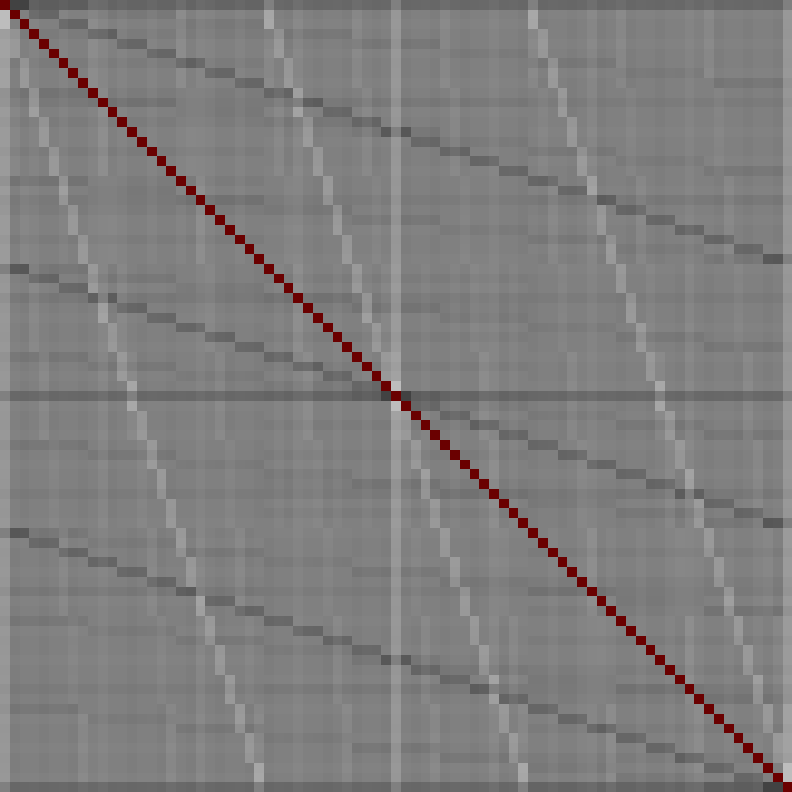
\includegraphics[width=0.5\linewidth]{s3k4}
	\caption{Table representing win probabilities in a game using a random outcome generator with three equally likely outcomes and players predicting the next four flips instead of the three in the basic variation. Again, the brighter a square is, the more likely the player whose sequences are represented by the rows is to win. In all games which are more complicated than the basic version, patterns begin to be visible.}
	\label{fig:s3k4}
\end{figure}

\begin{figure} [H]
	\centering
	\includegraphics[width=0.9\linewidth]{"s3k4 uneven"}
	\caption{The same situation as Figure \ref{fig:s3k4} except one outcome has a 50\% chance of occuring, another is 20\%, and another is 30\%. A new kind of pattern appears.}
	\label{fig:s3k4-uneven}
\end{figure}

The tool can also create tables for three-player games, but these need three-dimensional tables. The tools displays them in two-dimensional slices that users can scroll though. Additionally, there is an option to display the win probabilities of all players at once. The first, second, and third player's win probabilities are mapped to the colours red, green, and blue respectively, as can be seen in Figure \ref{fig:s3k4-3p}.

\begin{figure} [H]
	\centering
	\includegraphics[width=0.7\linewidth]{"s3k4 3p"}
	\caption{Table representing the same situation as Figure \ref{fig:s3k4} except there is a third player. This two-dimensional slice of the full table shows all games where the third player's chosen sequence is 1201. Notice that the patterns in red are identical to those in Figure \ref{fig:s3k4}, since red is showing the probability of Player 1 winning (the same thing that Figure \ref{fig:s3k4} shows), except now in a 3-player game.}
	\label{fig:s3k4-3p}
\end{figure}

The tool doesn't automatically visualize the whole three-dimensional table, but we manually created one in the 3d software Blender. A video showing off the render can be found at \href{https://github.com/Will-Drac/Penneys-Game/blob/main/paper/3d%20table%20render.mp4}{https://github.com/Will-Drac/Penneys-Game/blob/main/paper/3d\%20table\%20render.mp4}. Some images of it are shown in Figure \ref{fig:3d}.

\begin{figure} [H]
	\centering
	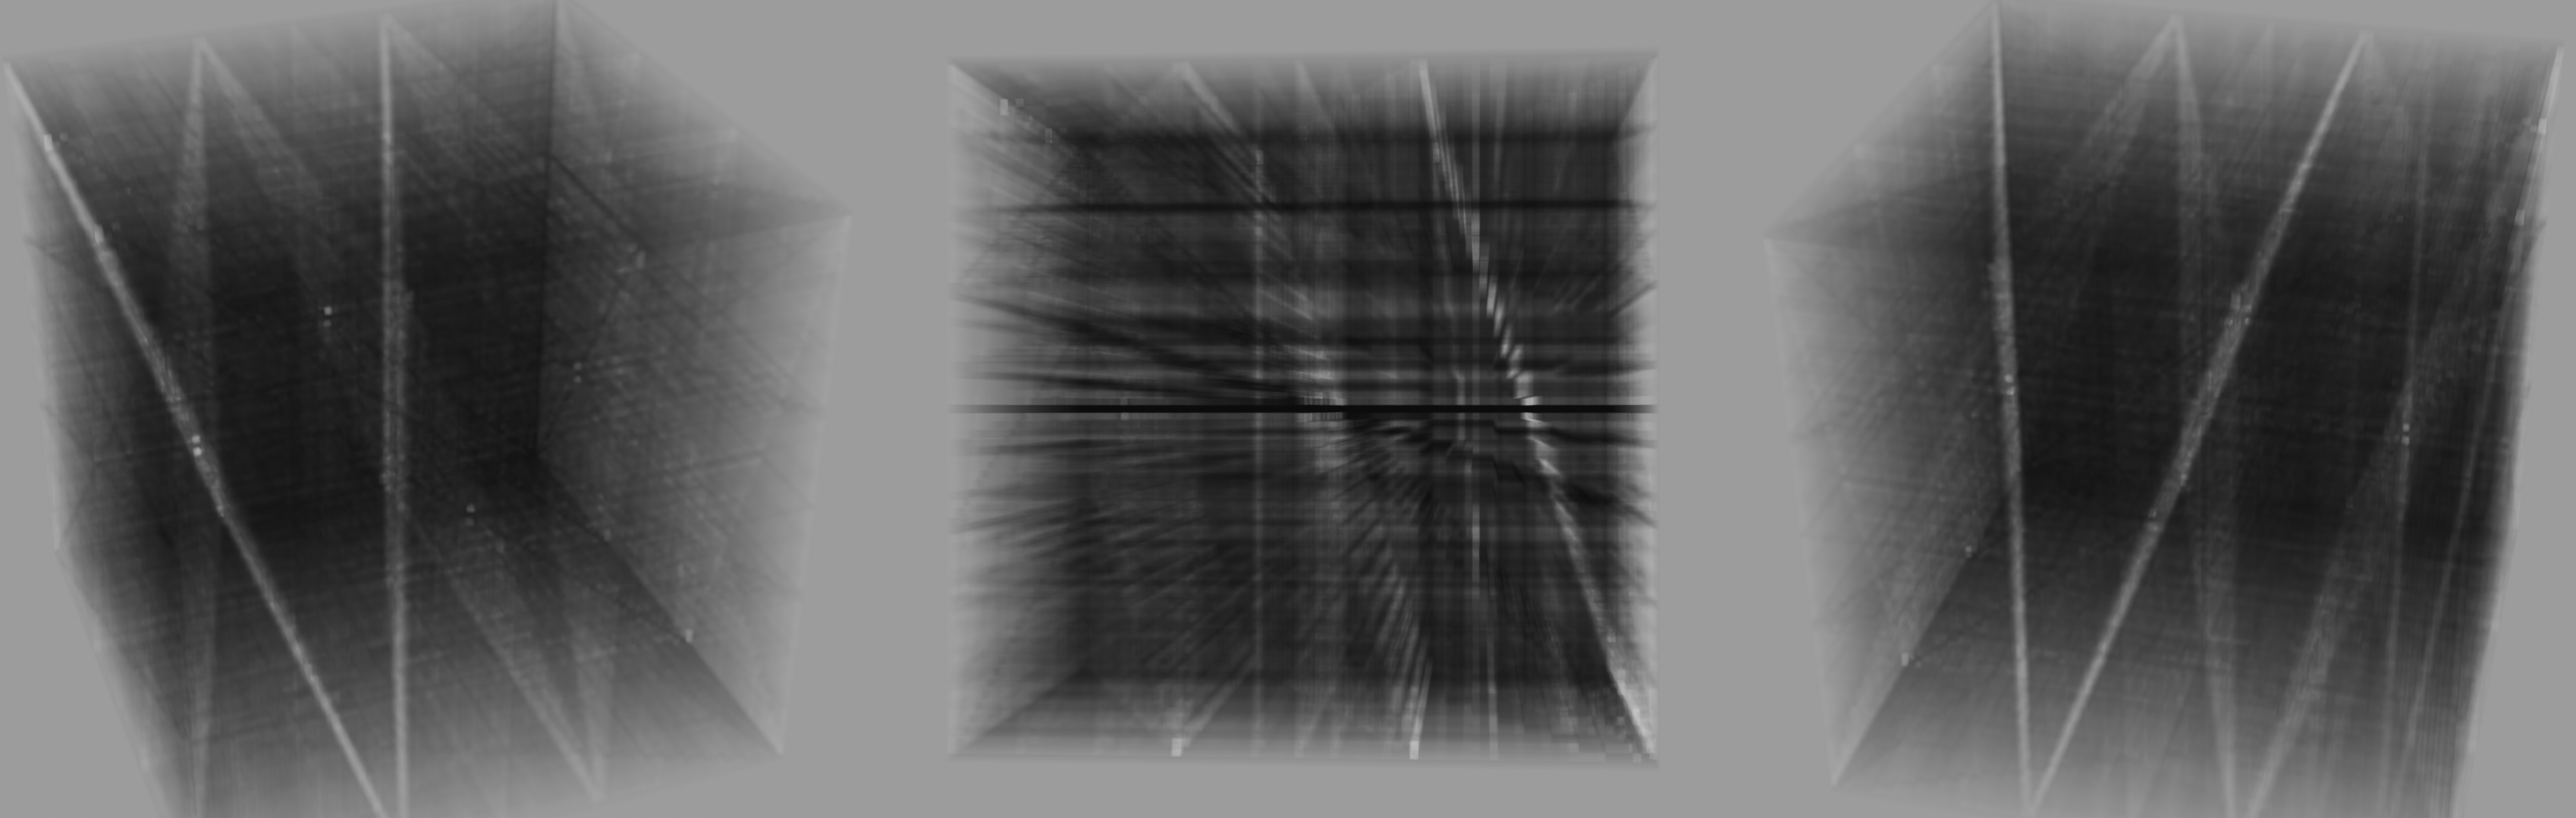
\includegraphics[width=0.9\linewidth]{3d}
	\caption{Visualization of a 3d win probabilities table from three different angles. The lighter a point is, the more likely the third player (the one with a new unique sequence for each slice on the upwards axis) is to win.}
	\label{fig:3d}
\end{figure}

The patterns in these tables tell us some new information about Penney's Game. Looking at Figure \ref{fig:s3k4}, we can notice three bright diagonal lines. These tell us that for each sequence that Player B chooses (each column), there are three sequences that Player A can choose (three rows) to get a high probability of winning (a bright square). The observation that the three appear right next to each other means that there is a pattern to them. This exact pattern is that the three sequences look like the opponent's sequence, except shifted over by one spot to the right. For example, if the opponent chooses \underline{120}2, the best strategy would be to pick a sequence X120. There is always a best choice for X, but there is seemingly no pattern in what it is. 

This shifting strategy is the same for any two-player game with equal sequence lengths and even flip outcome probabilities. With the correct $X$, it will produce the best response to any choice of sequence that an opponent might make.

The patterns in 3-player games are much more complicated and seem to interfere with each other so that there is no simple strategy.

\part {Physically modelling unfair coin flips and dice rolls \label{physicalModelling}}

Our equations can take into account random outcome generators with any probability distribution because of the $\mathbb{P}(Y_j)$ term in \eqref{Rdef}. We physically ground what this means by modelling the probability distribution of loaded dice and unfairly flipped coins.

\section{Deriving an approximate probability distribution for loaded dice}

Our goal in this section is to find a formula for the probability that a loaded die (a die with its centre of mass offset) lands on each of its faces. We will be making many key assumptions which are not true, but may be an accurate enough approximation.

\begin{enumerate}
	\item There is some point in the rolling of a die at which it is touching the table at one edge, without any rotational or translational motion. Imagine a die teetering on one edge, about to fall over so that it lands on a face but it hasn't started moving yet. This is pictured in Figure \ref{fig:loadeddie}.
	\item It is equally likely that a die lands as described in 1. on all edges.
	\item It is equally likely for a die to come at rest as described in 1. at any angle $\theta$ (as defined in Figure \ref{fig:loadeddie}).
\end{enumerate}

\begin{figure}[H]
	\centering
	\label{fig:loadeddie}
	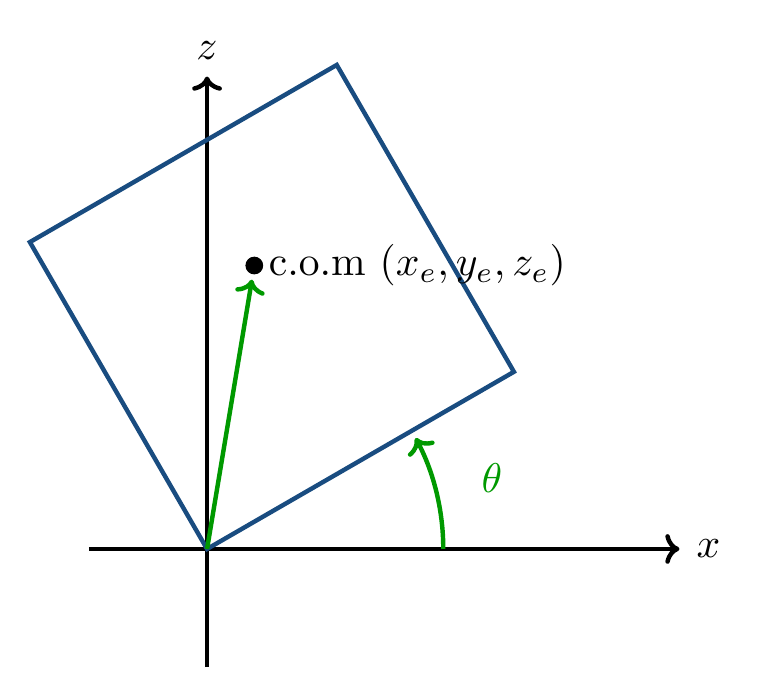
\begin{tikzpicture}[scale=6, every node/.style={scale=1.5}]
		\draw [->, ultra thick] (-0.25, 0) -- (1, 0) node[right] {$x$};
		\draw [->, ultra thick] (0, -0.25) -- (0, 1) node[above] {$z$};
		
		\begin{scope}[rotate=30]
			\draw[ultra thick, DarkBlue] (0, 0) -- (0.75, 0) -- (0.75, 0.75) -- (0, 0.75) --cycle;
		\end{scope}
		
		\filldraw [black] (0.1, 0.6) circle (0.5pt) node[right] { c.o.m $(x_e, y_e, z_e)$};
		
		\draw [->, ultra thick, OliveGreen] (0, 0) -- (0.095, 0.57);
		
		\draw [->, ultra thick, OliveGreen] (0.5, 0) arc (0: 28: 0.5);
		
		\draw (0.55, 0.15) node[right, OliveGreen] {$\theta$};
	\end{tikzpicture}
	
	\caption[A loaded die teetering on one of its edges]{A side view of a loaded die teetering on one of its edges. We are assuming that the die is currently at rest. Therefore, it will fall to whichever side the centre of mass (C.O.M) is on. In this case, it will rotate clockwise until it lands on the lower face.}
\end{figure}

Let's take the centre of mass to be at the point $(x_e, y_e, z_e)$ ($e$ indicating that it's the position when the die is aligned at an edge, as seen in Figure \ref{fig:loadeddie}). After a rotation by $\theta$, its new position $(x_{\theta}, y_{\theta}, z_{\theta})$ will be:

\begin{equation*}
	\begin{bmatrix} x_{\theta} \\ y_{\theta} \\ z_{\theta} \end{bmatrix} = \begin{bmatrix} \cos\theta & 0 & -\sin\theta \\ 0 & 1 & 0 \\ \sin\theta & 0 & \cos\theta \end{bmatrix} \begin{bmatrix} x_e \\ y_e \\ z_e \end{bmatrix}
\end{equation*}


Because of our assumptions, the probability that the die lands back on the face which makes $\theta = 0$ will be:

\begin{equation*}
	\mathbb{P} = \frac{\text{angles where the C.O.M will make it fall clockwise}}{\text{total angles possible}}
\end{equation*}

\begin{equation*}
	 \mathbb{P} = \frac{\text{angles where $x_{\theta} > 0$}}{\pi/2}
\end{equation*}

We can find which angles will make $x_{\theta} > 0$:

\begin{equation*}
	x' > 0
\end{equation*}
\begin{equation*}
	x_e\cos\theta - z_e\sin\theta > 0
\end{equation*}
\begin{equation*}
	\frac{x_e}{z_e} > \tan\theta
\end{equation*}

So it will fall back to $\theta=0$ for all $\theta < \arctan\mathlarger{\frac{x_e}{z_e}}$.

\begin{equation}\label{dieEdgeProb}
	\mathbb{P} = \frac{\arctan(x_e/z_e)}{\pi/2} = \frac{2}{\pi} \arctan\left(\frac{x_e}{z_e}\right)
\end{equation}

However, if we really want to find the probability of it landing on that face, we have to take into account that there are four edges which could possibly lead the die to fall onto that face. We can derive a formula which takes into account all four.

Let's imagine a die of side length $s$ and $r=\frac{s}{2}$. We will place the die on the xy-plane such that it is centred at $(0, 0, r)$. This is pictured in Figure \ref{fig:loadeddie3d}.

\begin{figure}[H]
	\centering
	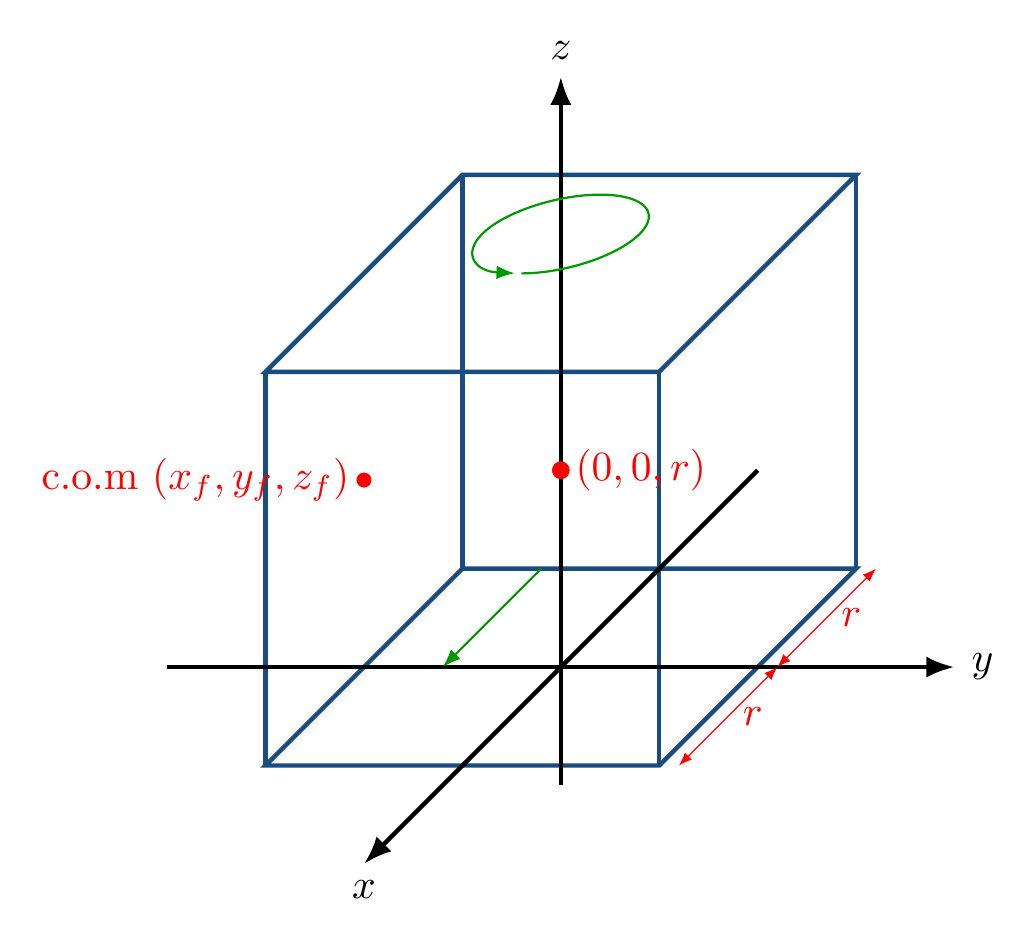
\begin{tikzpicture}[scale=2.5, 
		y={(1cm,0cm)}, z={(0cm,1cm)}, x={(-0.5cm,-0.5cm)},
		>=Latex, every node/.style={scale=1.5}]
		
		% cube
		\draw[ultra thick, DarkBlue] (-1,-1,0) -- (1,-1,0) -- (1,1,0) -- (-1,1,0) -- cycle; % bottom face
		\draw[ultra thick, DarkBlue] (-1,-1,2) -- (1,-1,2) -- (1,1,2) -- (-1,1,2) -- cycle; % top face
		\draw[ultra thick, DarkBlue] (-1,-1,0) -- (-1,-1,2);
		\draw[ultra thick, DarkBlue] (1,-1,0) -- (1,-1,2);
		\draw[ultra thick, DarkBlue] (1,1,0) -- (1,1,2);
		\draw[ultra thick, DarkBlue] (-1,1,0) -- (-1,1,2);
		
		% axes
		\draw[->, ultra thick] (-2,0,0) -- (2,0,0) node[below] {$x$};
		\draw[->, ultra thick] (0,-2,0) -- (0,2,0) node[right] {$y$};
		\draw[->, ultra thick] (0,0,-0.6) -- (0,0,3) node[above]{$z$};
		
		% COM marker
		\filldraw[red] (0.5,-0.75,1.2) circle (1pt) node[left] {c.o.m $(x_f,y_f,z_f)$};
		
		% center marker
		\filldraw[red] (0,0,1) circle (1.2pt) node[right] {$(0,0,r)$};
		
		% r measurements
		\draw[red, <->] (-1,1.1,0) -- (0,1.1,0);
		\node[red, right] at (-0.5, 1.1, 0) {$r$};
		
		\draw[red, <->] (0,1.1,0) -- (1,1.1,0);
		\node[red, right] at (0.5, 1.1, 0) {$r$};
		
		% green rotation arrow on the z-axis
		\draw[OliveGreen, ->, thick] (0.4,0,2.2) arc (0:355:0.4);
		
		% green movement arrow towards +x
		\draw[OliveGreen, ->, thick] (-1, -0.6, 0) -- (0,-0.6,0);
		
	\end{tikzpicture}
	\caption{Setup for calculating the probability of a loaded dice landing on the down-facing "selected face". The green arrows represent the rotation and translation which are used to line up the selected edge with the y-axis.}
	\label{fig:loadeddie3d}
\end{figure}

For each edge of the selected face (let's call it the "selected edge"), we will:

\begin{enumerate}
	\item Rotate the die so that the selected edge is centred on $(-r, 0, 0)$ and parallel to the y-axis.
	\item Translate the die forward in the x-direction so that the edge is centred at the origin. We now have the situation in Figure \ref{fig:loadeddie} for our selected face but with $\theta=0$ because we haven't started checking the angles yet.
	\item Determine the probability that it lands on the selected (down-facing) face using \eqref{dieEdgeProb}.
	\item Mix the probabilities from each selected edge to get the final probability of the die landing on the selected face.
\end{enumerate}

From steps 1. and 2., we must rotate the centre of mass $(x_f, y_f, z_f)$ ($f$ indicating that it's the position when the die is aligned at a face, as seen in Figure \ref{fig:loadeddie3d}) and then translate it to follow the die being rotated and translated. The C.O.M will end up at $(x_e, y_e, z_e)$ because the die will be oriented like in Figure \ref{fig:loadeddie}.

\begin{equation*}
	\begin{bmatrix}x_e\\y_e\\z_e\end{bmatrix} = \begin{bmatrix}\cos\phi & -\sin\phi & 0 \\ \sin\phi & \cos\phi & 0 \\ 0 & 0 & 1\end{bmatrix} \begin{bmatrix}x_f\\y_f\\z_f\end{bmatrix} + \begin{bmatrix}r\\0\\0\end{bmatrix}
\end{equation*}

So \eqref{dieEdgeProb} with $(x_e, y_e, z_e)$ in terms of $(x_f, y_f, z_f)$ is:

\begin{equation*}
	\mathbb{P} = \frac{2}{\pi}\arctan\left(\frac{x_e}{z_e}\right) = \frac{2}{\pi}\arctan\left(\frac{x_f\cos\phi-y_f\sin\phi+r}{z_f}\right)
\end{equation*}

If the die starts as it is in Figure \ref{fig:loadeddie3d}, we have one edge which requires no rotation to get selected ($\phi=0$ will have it oriented properly) and three other edges, each with an additional rotation of $\frac{\pi}{2} \text{rad}$ relative to the previous. To model this, we let $\phi = n\pi/2 \text{ with } n=\{0, 1, 2, 3\}$ to cover all four edges being selected.

Additionally, we are assuming that there is equal likelihood that the die lands on each of the 12 edges, so the chance that it lands on any one of the edges is $\frac{1}{12}$. The contribution to the probability that the die lands on the selected face coming from the selected edge is:

\begin{equation*}
	\mathbb{P}_n = \frac{1}{12} \cdot \frac{2}{\pi} \arctan\left(\frac{x_f\cos(n\frac{\pi}{2})-y_f\sin(n\frac{\pi}{2})+r}{z_f}\right)
\end{equation*}

Finally, the total probability of the die landing on the selected face is the sum of the contributions by each edge of that face:

\begin{equation}\label{dieFaceProb}
	\mathbb{P}_F = \frac{1}{6\pi} \sum_{n=0}^{3} \arctan\left(\frac{x_f\cos(n\frac{\pi}{2})-y_f\sin(n\frac{\pi}{2})+r}{z_f}\right)
\end{equation}

One last thing must be done, since we want a single formula which returns the probability for all sides of a die. We need a procedure to align the die as it is in Figure \ref{fig:loadeddie3d} for all faces, so that any face may be selected.

We imagine the die centred at the origin with the symbol "1" facing towards $-z$, "2" facing towards $+x$, and "3" facing towards $+y$. The centre of mass $(x_o, y_o, z_o)$ ($o$ indicating that it's the position when the die is aligned at the origin) will be defined according to that coordinate system. For each face, indexed by $F \in [1, 6] $, we will define three angles $\alpha$, $\beta$, $\gamma$ which will get the die to rotate so that the selected face is pointing to $-z$. The rotation will be followed by a translation to shift the centre of the die to be like it is in Figure \ref{fig:loadeddie3d}.

\begin{equation*}
	\alpha = \begin{cases} 
		0 & \text{ if } F \le 2 \\
		-\pi/2 & \text{ if } F = 3 \\
		-3\pi/2 & \text{ if } F = 4 \\
		-\pi & \text{ if } F \ge 5  \\
	\end{cases}
\end{equation*}

\begin{equation*}
	\beta = \begin{cases} 
		0 & \text{ if } F = 1 \text{ or } F = 6 \\
		\pi/2 & \text{ otherwise }
	\end{cases}
\end{equation*}

\begin{equation*}
	\gamma = \begin{cases} 
		0 & \text{ if } F \le 3 \\
		\pi/2 & \text{ if } F \ge 4
	\end{cases}
\end{equation*}	

So now we can define the position of the center of mass $(x_f, y_f, z_f)$ in \eqref{dieFaceProb} as a function of the face selected and the position of the centre of mass in the coordinate system described in the previous paragraph: $(x_o, y_o, z_o)$.

\begin{equation*}
	\begin{bmatrix}
		x_f \\ y_f \\ z_f
	\end{bmatrix}
	=
	\begin{bmatrix}
		\cos\gamma & -\sin\gamma & 0 \\
		\sin\gamma & \cos\gamma & 0 \\
		0 & 0 & 1
	\end{bmatrix}
	\begin{bmatrix}
		1 & 0 & 0 \\
		0 & \cos\alpha & -\sin\alpha \\
		0 & \sin\alpha & \cos\alpha
	\end{bmatrix}
	\begin{bmatrix}
		\cos\beta & 0 & \sin\beta \\
		0 & 1 & 0 \\
		-\sin\beta & 0 & \cos\beta
	\end{bmatrix}
	\begin{bmatrix}
		x_o \\ y_o \\ z_o
	\end{bmatrix}
	 +
	 \begin{bmatrix}
	 	0 \\ 0 \\ r
	 \end{bmatrix}
\end{equation*}

And in the end, we have a function (which is too big to be fully written out), which inputs $(x_o, y_o, z_o)$ and the side length of the die $s$ and outputs a probability for each outcome of rolling the die. The outcomes are indexed with the variable $F$, which represents the number on the die that will end up flat against the table. To retrieve the probability of a face ending up facing upwards (let's label it $F'$), use the function with $F=7-F'$, since numbers on opposite faces of a die add up to 7.

$\mathbb{P}_F$ would be used as our value for $\mathbb{P}(Y_j)$.

\section{Simulating an unfair coin flip}

\textcite{unfairCoin} describe a way to flip a coin which makes it more likely to land on a particular side. Put simply, if a coin is spun like a flying disc, the side which started facing upwards will stay that way. In Theorem 2, Diaconis \textit{et al.} provide a formula for the probability that the coin lands on the upward-facing side as a function of the angle between the normal direction of the coin and its axis of rotation $\psi$:

\begin{equation}\label{coinProbByAngle}
	p = \begin{cases}
		\frac{1}{2} + \frac{1}{\pi}\arcsin(\cot^2(\psi)) & \text{ if } \frac{\pi}{4}<\psi<\frac{3\pi}{4}
		\\
		1 & \text{ if } 0<\psi<\frac{\pi}{4} \text{ or } \frac{\pi}{4} < \psi < \pi
	\end{cases}
\end{equation}

$p$ would be used as our value for $\mathbb{P}(Y_j)$. To add on to their work, we created a flipping coin simulator which demonstrates the phenomenon they describe. The simulator can be found at \href{https://will-drac.github.io/Penneys-Game/flipping%20coin/}{will-drac.github.io/Penneys-Game/flipping\%20coin/}

\begin{figure}[H]
	\centering
	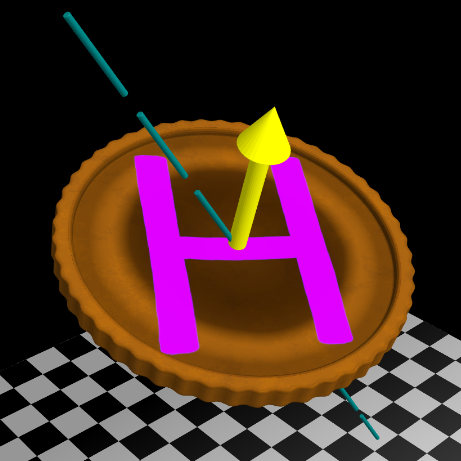
\includegraphics[width=0.7\linewidth]{flippingCoin}
	\caption{Freeze frame of the simulator, showing the coin's normal in yellow and the axis of rotation in cyan. As described by Diaconis \textit{et al.}, the normal rotates about the axis.}
	\label{fig:flippingcoin}
\end{figure}

\subsection{Finding the force to apply to the coin as a function of the coin's desired probability}

Another addition to \textcite{unfairCoin}'s work is a derivation of the force vector required to give the coin a particular probability.

Inverting \eqref{coinProbByAngle}, we get the angle between the coin's normal direction and its rotational axis ($\psi$) as a function of the probability it produces ($p$):

\begin{equation}\label{coinAngleByProb}
	\psi(p) = \arctan\left(\left[\sin(\pi p-\frac{\pi}{2})\right]^{-\frac{1}{2}}\right) \text{ for } p \in \left[\frac{1}{2}, 1\right]
\end{equation}

We imagine a coin with mass $M$ and radius $R$ receiving a force $\vec{F}$ which is anywhere except at the coin's centre (because that would result in no rotation), and the force having a large enough magnitude that the coin will make enough flips in the air so that the outcome is really random. We define a coordinate system as seen in Figure \ref{fig:coincoords}. The surface normal of the coin before being flipped is made to be $\hat{n} = <0, 0, 1>$.

\begin{figure}[H]
	\centering
	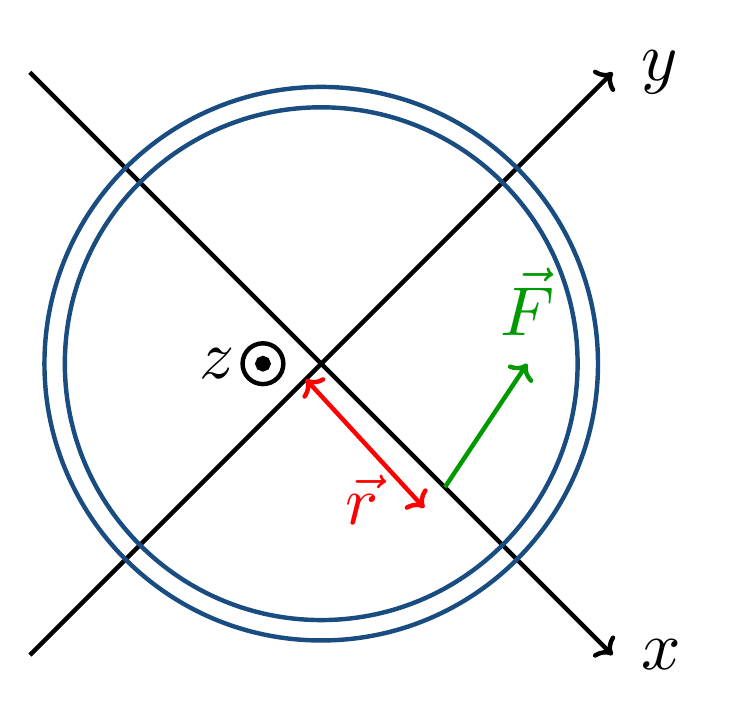
\begin{tikzpicture}[scale=3.7, ultra thick, every node/.style={scale=2.5}]
		\draw [->] (-1, 1) -- (1, -1) node[right] {$x$};
		
		\draw [->] (-1, -1) -- (1, 1) node[right] {$y$};
		
		\filldraw (-0.2, 0) circle (0.55pt) node[left] {$z$};
		
		\draw (-0.13, 0) arc (0:360:0.07); 
		
		\draw [DarkBlue] (0.95, 0) arc (0:360:0.95);
		\draw [DarkBlue] (0.88, 0) arc (0:360:0.88);
		
		\begin{scope}[rotate=-45]
			\draw [<->, red] (0, -0.075) -- (0.6, -0.1);
			\node [red, below] at (0.3, -0.1) {$\vec{r}$};
			
			\draw [->, OliveGreen] (0.6, 0) -- (0.5, 0.5) node[above] {$\vec{F}$};
		\end{scope}
	\end{tikzpicture}
	\caption{Coordinate system set up to determine the force vector $\vec{F}$ required to give the coin a particular probability $p$. The origin is placed at the centre of the coin and the point at which the force is applied lies on the x-axis.}
	\label{fig:coincoords}
\end{figure}

We imagine the constant force $\vec{F}$ being applied to a motionless coin for a short period of time $\Delta t$. Ignoring the linear motion that this would induce, since it would only affect the path of the coin in the air and not the flip, we can find the torque $\vec{\tau}$ that the force applies to the coin:

\begin{equation*}
	\vec{\tau} = \vec{r}\times\vec{F} = \begin{bmatrix}r\\0\\0\end{bmatrix} \times \begin{bmatrix}F_x \\ F_y \\ F_z\end{bmatrix} = r\begin{bmatrix}0\\-F_z\\F_y\end{bmatrix}
\end{equation*}

The torque gives the coin some angular momentum $\vec{L}$:

\begin{equation*}
	\vec{\tau} \cdot \Delta t = r \Delta t\begin{bmatrix}0\\- F_z \\ F_y \end{bmatrix} = \vec{L}
\end{equation*}

From the angular momentum, we can get the angular velocity $\vec{\omega}$, which is in the direction of the axis of rotation.

\begin{equation*}
	\vec{L} = \mathbf{I} \vec{\omega} \implies \mathbf{I}^{-1} \vec{L} = \vec{\omega}
\end{equation*}

Since $\vec{L}$ can be in any direction, the moment of inertia $\mathbf{I}$ must be in its most general form: a matrix. We are assuming that the coin's thickness is negligible compared to its radius when calculating $\mathbf{I}$.

\begin{equation*}
	\mathbf{I}
	=
	\begin{bmatrix}
		I_{xx} & I_{xy} & I_{xz} \\
		I_{yx} & I_{yy} & I_{yz} \\
		I_{zx} & I_{zy} & I_{zz} \\
	\end{bmatrix}
	=
	\frac{MR^2}{4}
	\begin{bmatrix}
		1 & 0 & 0 \\
		0 & 1 & 0 \\
		0 & 0 & 2 \\
	\end{bmatrix}
	\implies
	\mathbf{I}^{-1}
	=
	\frac{4}{MR^2}
	\begin{bmatrix}
		1 & 0 & 0 \\
		0 & 1 & 0 \\
		0 & 0 & \frac{1}{2} \\
	\end{bmatrix}
\end{equation*}

\begin{equation*}
	\mathbf{I}^{-1} \vec{L} = \frac{4r\Delta t}{MR^2} \begin{bmatrix}0\\- F_z \\ \frac{F_y}{2} \end{bmatrix} = \vec{\omega}
\end{equation*}

Since $\psi$ is defined as the angle between the normal $\hat{n}$ and the axis of rotation (which is parallel to $\vec{\omega}$), it can be calculated like so:

\begin{equation*}
	\hat{n} \cdot \vec{\omega} = |\hat{n}| |\vec{\omega}| \cos\psi \implies \psi = \arccos\left(\frac{\hat{n}\cdot\vec{\omega}}{|\vec{\omega}|}\right)
\end{equation*}

\begin{equation*}
	\psi = \arccos \left(\frac{F_y/2}{\sqrt{(F_z)^2+(\frac{F_y}{2})^2}}\right) = \arctan\left(\frac{2F_z}{F_y}\right)
\end{equation*}

A general form of a function for $\vec{F}$ which satisfies $\psi = \arctan\left(\frac{2F_z}{F_y}\right)$ is

\begin{equation*}
	\vec{F}(p) = \begin{bmatrix}a\\2b\cos\left(\psi\right)\\b\sin\left(\psi\right)\end{bmatrix}
\end{equation*}

With $a$ being any real number and $b$ being any non-zero real number. Substituting $\psi$ with \eqref{coinAngleByProb}, we get $\vec{F}$ as a function of $p$.

\part {Conclusion}

We successfully extended the analogy of the betting game and created a formula for probability of each player winning in many variations of Penney's Game: games with any number of players, players predicting any number of flips even if they are different to each other, any kind of random outcome generator, and any probability distribution for the random outcome generator. We then physically modelled what it means to have a skewed probability distribution on dice and coins. We also created a simulator which was able to verify our results beyond doubt. Finally, we developed a software tool which helped us to determine other trends and patterns in the game: the game limits to being fair as the number of possible outcomes of the flip tends to infinity but not as sequence length tends to infinity in two-player games, there is a general strategy for two-player games, and the shorter sequence in two-player games always has an advantage, except in a few known cases.

\section{Acknowledgements}

A huge thanks to the supervisor for this project, Derrick Chung, for guiding the research while leaving plenty of room to explore. His experience and advice proved extremely valuable. Another big thanks goes to Dr. Ferenc Balogh for coordinating the Independent Research Project in Science course here at John Abbott College. None of this would have been possible without both of these great people.

\part {References}
\printbibliography[heading=none]



\end{document}